\documentclass[tikz,crop]{standalone}

\usepackage{tikz}
\usepackage{xcolor}
\usepackage{pgfplots}
\usepackage{scratch3}
\usepackage{siunitx}
%\usepackage{tikz-uml}

\pgfplotsset{compat=1.18}
\usepgfplotslibrary{statistics}

\usetikzlibrary{shapes,arrows,positioning,backgrounds,calc,intersections,calc,svg.path,fit}

\definecolor{ugent-re}{RGB}{220, 78, 40}        % vermilion			/ vermiljoen
\definecolor{ugent-we}{RGB}{45, 140, 168}       % no match
\definecolor{ugent-ge}{RGB}{232, 94, 113}       % rose				/ bleekrood
\definecolor{ugent-ea}{RGB}{111, 113, 185}      % distant blue		/ verblauw
\definecolor{ugent-pp}{RGB}{251, 126, 58}       % deep orange		/ dieporanje
\definecolor{ugent-ps}{RGB}{113, 168, 96}       % yellow green		/ geelgroen

\tikzstyle{python}=[fill=ugent-ps!50!white]
\tikzstyle{java}=[fill=ugent-we!50!white]
\tikzstyle{haskell}=[fill=ugent-ea!50!white]
\tikzstyle{js}=[fill=ugent-pp!50!white]
\tikzstyle{c}=[fill=ugent-re!50!white]

\newlength{\block}
\setlength{\block}{0.75cm}

\tikzstyle{a}=[anchor=north west]
\tikzstyle{box}=[a,draw,rectangle]
\tikzstyle{node}=[a,draw,minimum height=0.5cm,align=center,fill=white,text depth=.25ex]
\tikzstyle{document}=[node,tape,tape bend top=none]
\tikzstyle{cont}=[box,minimum height=1\block,minimum width=1\block]
\tikzstyle{arrow}=[draw, -latex]
\tikzstyle{inner}=[box,draw=gray]

% Blue box style
\tikzstyle{bluebox}=[draw=ugent-we,java]
\tikzstyle{redbox}=[draw=ugent-re,c]
\tikzstyle{greenbox}=[draw=ugent-ps,python]

% Some things specific to TESTed imagery.
\tikzstyle{tc}=[box,draw=ugent-ps]
\tikzstyle{comp}=[box,draw=ugent-re,fill=ugent-re,fill opacity=0.05]
\tikzstyle{exec}=[box,draw=ugent-we,fill=ugent-we,fill opacity=0.10]

% Stuff from tested-engine/concept.tex
\tikzstyle{process}=[node,rectangle]
\tikzstyle{terminator}=[node,rectangle,rounded corners=0.5cm]
\tikzstyle{io}=[node,trapezium,trapezium left angle=70,trapezium right angle=-70,minimum width=2.5cm,trapezium stretches=true]
\tikzstyle{small}=[font=\footnotesize,color=darkgray]
\tikzstyle{submission}=[document,align=right,minimum width=3cm,minimum height=1cm,text depth=0.5cm,inner sep=0.5mm,font=\scriptsize]

% Stuff from chatper3/flow.tex
\tikzstyle{height}=[minimum height=0.75\block]
\tikzstyle{contt}=[cont,minimum height=0.75\block]
\tikzstyle{compop}=[comp,text opacity=1]
\tikzstyle{execop}=[exec,text opacity=1]

\tikzstyle{hnode}=[draw,anchor=center,minimum height=\block,text depth=.25ex,align=center]
\tikzstyle{executable}=[hnode,ultra thick,fill=gray!10]
\tikzstyle{inner-exec}=[node,anchor=center,minimum width=3.25\block,densely dotted,font=\footnotesize,fill=none]
\tikzstyle{stmt}=[node,anchor=center,fill=gray!30,minimum width=4.5\block,font=\footnotesize]
\tikzstyle{fieldset}=[minimum height=\block,fill=white,text depth=.5ex,fill=white]

\begin{document}

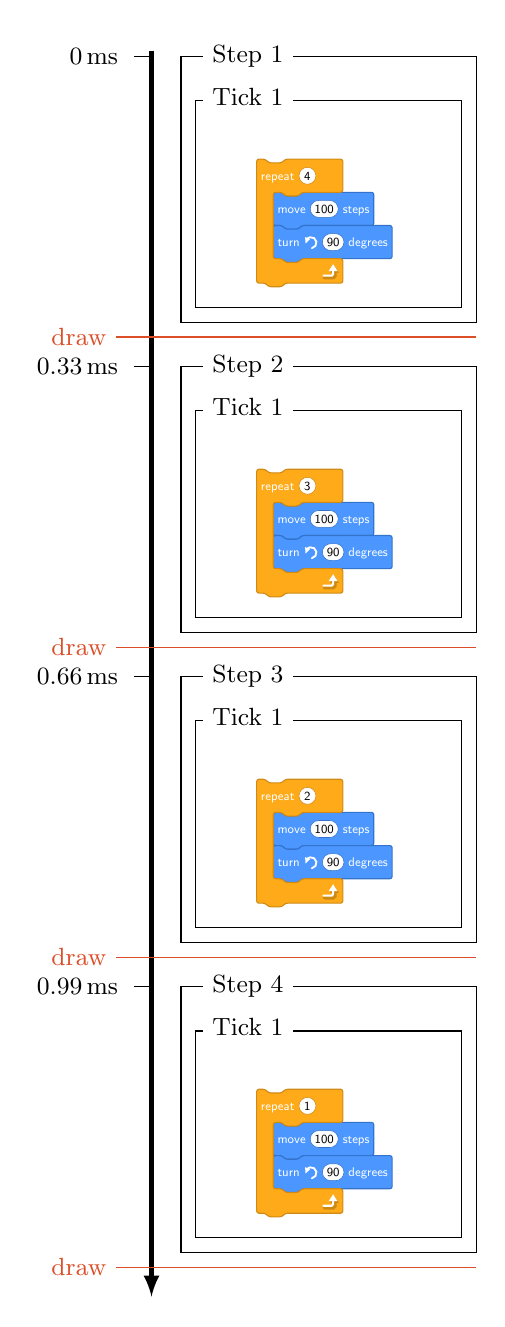
\begin{tikzpicture}[x=0.75cm,y=0.75cm,every node/.style={font=\small}]

  \draw[arrow, ultra thick] (0,0.1) -- (0,-21);

  % Draw horizontal lines
  \foreach \y [count=\yi] in {0,5.25,10.5,15.75} {
    \node[draw=none,anchor=east] at (-0.4,-\y) {\qty[evaluate-expression]{\fpeval{(\yi-1)*0.33}}{\milli\second}};
    \draw (-0.3,-\y) -- (0,-\y);
  }

  \foreach \y [count=\yi] in {4.75,10,15.25,20.5} {
    \draw [ugent-re] (-0.6,-\y) -- (5.5,-\y);
    \node[anchor=east,text=ugent-re] at (-0.6,-\y) {draw};
  }

  \node[hnode, minimum height=4.5\block, minimum width=5\block,label={[fieldset,above left=-0.53\block and 0.6\block]Step 1}] at (3,-2.25) {};
  \node[hnode, minimum height=3.5\block, minimum width=4.5\block,label={[fieldset,above left=-0.5\block and 0.6\block]Tick 1}] at (3,-2.5) {
    \begin{scratch}[scale=0.5,baseline=3]
      \blockrepeat{repeat \ovalnum{4}}{
        \blockmove{move  \ovalnum{100} steps}
        \blockmove{turn \turnleft{} \ovalnum{90} degrees}
      }
    \end{scratch}
  };

  \node[hnode, minimum height=4.5\block, minimum width=5\block,label={[fieldset,above left=-0.53\block and 0.6\block]Step 2}] at (3,-7.5) {};

  \node[hnode, minimum height=3.5\block, minimum width=4.5\block,label={[fieldset,above left=-0.5\block and 0.6\block]Tick 1}] at (3,-7.75) {
    \begin{scratch}[scale=0.5,baseline=3]
      \blockrepeat{repeat \ovalnum{3}}{
        \blockmove{move  \ovalnum{100} steps}
        \blockmove{turn \turnleft{} \ovalnum{90} degrees}
      }
    \end{scratch}
  };

  \node[hnode, minimum height=4.5\block, minimum width=5\block,label={[fieldset,above left=-0.53\block and 0.6\block]Step 3}] at (3, -12.75) {};

  \node[hnode, minimum height=3.5\block, minimum width=4.5\block,label={[fieldset,above left=-0.5\block and 0.6\block]Tick 1}] at (3, -13) {
    \begin{scratch}[scale=0.5,baseline=3]
      \blockrepeat{repeat \ovalnum{2}}{
        \blockmove{move  \ovalnum{100} steps}
        \blockmove{turn \turnleft{} \ovalnum{90} degrees}
      }
    \end{scratch}
  };

  \node[hnode, minimum height=4.5\block, minimum width=5\block,label={[fieldset,above left=-0.53\block and 0.6\block]Step 4}] at (3, -18) {};

  \node[hnode, minimum height=3.5\block, minimum width=4.5\block,label={[fieldset,above left=-0.5\block and 0.6\block]Tick 1}] at (3, -18.25) {
    \begin{scratch}[scale=0.5,baseline=3]
      \blockrepeat{repeat \ovalnum{1}}{
        \blockmove{move  \ovalnum{100} steps}
        \blockmove{turn \turnleft{} \ovalnum{90} degrees}
      }
    \end{scratch}
  };
\end{tikzpicture}

\end{document}
